\documentclass[a4paper,10pt]{article}

\usepackage{polski}
\usepackage[latin2]{inputenc}
\usepackage{makeidx}
\usepackage{graphicx}
\usepackage{moreverb}
\usepackage{listings}

%============================= Definicje makr=============================
% finicja naglowka posrodku strony
\newcommand{\nagl}[1]{\par\begin{center}{\bf{#1}}\end{center}\par}
% Definicja tego na poczatku
\newcommand{\pocz}{\par {\bf{\nazwaprojektu}}\par {\bf{\nazwadokumentu}}\par {\bf{Wersja: \wersjadokumentu}}\par} 
%% Historia
% environment
\newenvironment{historia}{\nagl{Historia}\begin{tabular*}{17cm}{c|c|c|l} {\bf{Data}} & {\bf{Wersja}} & {\bf{Autor}} & {\bf{Zmiany}} \\}{\end{tabular*}}
% item
\newcommand{\hist}[4]{#1 & #2 & #3 & \parbox[t]{8cm}{#4} \\ }

% Marginesy
\textwidth17cm \textheight24.5cm \topmargin-40pt
\oddsidemargin-0.04cm
%=========================================================================

\makeindex 
 
\newcommand{\nazwaprojektu}{ProtoGen 1.0}
\newcommand{\nazwadokumentu}{Dokumentacja generatora protoko��w sieciowych} 

\newcommand{\wersjadokumentu}{0.8}


%% Tabelka o znaczeniu poszczeg�lnych bajt�w w protokole
\newenvironment{bajty}{\\ \begin{tabular}{|l|l|l|}\hline
{\bf{Od - do}} & {\bf{Typ/Warto��}} & {\bf{Zawarto��}} \\\hline}{\hline\end{tabular}\\\\} % item


\newcommand{\bp}[4]{\parbox[t]{2.5cm}{#1 $\rightarrow$ #2} & \parbox[t]{3cm}{#3\\} & \parbox[t]{10cm}{#4\vspace{1em}}
\\ } 

\newcommand{\znacznik}[1]{$<$#1$>$}

\title{\nazwaprojektu \ --- \nazwadokumentu}
\author{Piotr Tabor (pt214569@students.mimuw.edu.pl)}


\begin{document}
\maketitle

\begin{historia}
	\hist{2008-05-22}{0.1}{Piotr Tabor}{Pierwsza wersja dokumentu}
	\hist{2008-05-25}{0.2}{Piotr Tabor}{Sko�czona dokumentacja formatu XML
	opisuj�cego protok�}
	\hist{2008-05-26}{0.3}{Piotr Tabor}{Spisane pozosta�e rozdzia�y}
	\hist{2008-05-27}{0.4}{Piotr Tabor}{Poprawienie liter�wek}
	\hist{2008-05-27}{0.5}{Piotr Tabor}{Poprawienie wed�ug uwaga dr hab.
	Krzysztofa Stencla, dopisanie przyk�ad�w u�ycia}
	\hist{2008-05-27}{0.6}{Piotr Tabor}{Przejrzenie i poprawki ca�o�ci}
	\hist{2008-05-28}{0.7}{Piotr Tabor}{Dodanie informacji o typie
	,,bytes'' (\ref{bytes})}
	\hist{2008-06-01}{0.8}{Piotr Tabor}{Dodanie schematu XML deskryptora w dodatku:
	\ref{xml-schema}}
\end{historia}

\tableofcontents

\newpage

	\section{Wprowadzenie}

\subsection{Wst�p}

Generator protoko��w jest narz�dziem s�u��cym do generowania implementacji
protoko�u sieciowego w r�nych j�zykach programowania w oparciu o zadany opis. 
Danymi wej�ciowymi generatora jest specyfikacja protoko�u zapisana w pliku XML
(patrz: \ref{xml}) oraz wybrany j�zyk programowania. Danymi wyj�ciowymi jest 
kod �r�d�owy w wybranym j�zyku programowania umo�liwiaj�cy wygodne pos�ugiwanie
si� tym protoko�em.

\subsection{Licencjonowanie}

Projekt ,,ProtoGen 1.0'' jak i wygenerowany przez niego kod jest licencjonowany
na zasadach licencji ,,Apache Software License 2.0''
(http://www.apache.org/licenses/LICENSE-2.0).

\subsection{Korzy�ci p�yn�ce ze stosowania tego rozwi�zania}

Zastosowanie tego narz�dzia daje nast�puj�ce korzy�ci:
\begin{itemize}
  \item Gwarantuje zgodno�� na poziomie danych przysy�anych sieci� dla
  implementacji w r�nych j�zykach programowania
  \item Pozwala unikn�� programi�cie ,,mechanicznego'' tworzenia du�ych ilo�ci
  kodu a zaraz b��d�w z tym zwi�zanych
  \item Gwarantuje, �e ca�y kod protoko�u jest napisany w spos�b sp�jny
  \item Gwarantuje, �e wygenerowany kod jest odporny na podstawowe zagro�enia w
  komunikacji pomi�dzy r�nymi architekturami: problem kolejno�ci bajt�w w
  s�owie (big-endian/little-endian) oraz problem rozmiaru podstawowych typ�w
  danych (architektury od 8 do 64 bit�w).
  \item Tworzy zestawy test�w, kt�re
  umo�liwiaj� sprawdzanie komunikacji tak�e pomi�dzy kodem wygenerowanym dla
  r�nych j�zyk�w programowania. 
  \item Umo�liwia aktualizacj� ca�ego modu�u poprzez aktualizacj� generatora i
  ponowne wygenerowanie kodu. 
\end{itemize}

\subsection{Ograniczenia rozwi�zania}

ProtoGen nie jest narz�dziem, kt�re umo�liwia wygenerowanie modu�u
obs�uguj�cego ka�dy protok�. W obecnej wersji zosta�y przyj�te poni�sze
ograniczenia.

\subsubsection{Budowa paczki}

		Ka�da paczka ma nast�puj�cy schemat budowy:
		\begin{bajty}
                	\bp{0}{$a$}{'zale�y od konfiguracji'}{Sta�a m�wi�ca o typie
                	paczki, a tym samym okre�laj�ca format zawartych w nich danych}
                	\bp{$a+1$}{$a+4$}{uint32}{n- Sta�a okre�laj�ca
                	ilo��
                	danych w�a�ciwych zawartych w paczce - wyra�ona w bajtach}
                	\bp{$a+5$}{$a+5+n$}{patrz opis zale�ny od typu paczki}{Dane
                	w�a�ciwe paczki zgodne z formatem okre�lonym poprzez typ paczki}
 		    \end{bajty}	
		Formalnie b�dziemy m�wili, �e paczka si� sk�ada z dwu-polowego nag��wka oraz
		cia�a. Nag��wek wyznacza typ paczki i rozmiar danych w�a�ciwych w niej
		zawartych, a cia�o - to dane interpretowane zale�nie od typu paczki. 
		
		
\subsubsection{Big/endian - little/endian}
Przyj�to, �e wszystkie dane s� przesy�ane przez sie� w formacie big-endian.

\subsubsection{Format napis�w}
Przyj�to, �e wszystkie napisy s� przesy�ane przez sie� w formacie UTF-8. 

\subsection{Z�o�ona logika}
	
	Obecnie ProtoGen nie wspiera z�o�onej logiki w konstrukcji pakiet�w. Niemo�liwe jest warunkowanie istnienia pola w zale�no�ci od warto�ci innego pola,
	a tak�e tworzenia tablicy p�l. Obecnie ProtoGen przewiduje mo�liwo��
	nadpisania wygenerowanego kodu. W ten spos�b - nadpisuj�c kod obs�ugi
	odpowiedniej paczki - mo�na uzyska� obs�ug� dowolnie z�o�onej logiki.

	O planowanym rozwi�zaniu tego problemu w przysz�ych wersjach mo�esz przeczyta�
	w rozdziale ,,Dalszy rozw�j'' (patrz: \ref{roadmap})		 	

\newpage
\section{Dokumentacja u�ytkownika}
	\subsection{Uruchomienie}
	
	ProtoGen uruchamiamy b�d�c w katalogu w kt�rym znajduj� si� jego pliku
	uruchomieniowe. W zale�no�ci od systemu operacyjnego uruchamiamy protoGen.sh
	(UNIXy), b�d� protoGen.bat (MS Windows) podaj�c nast�puj�ce parametry:
	\begin{description}
		\item[�cie�ka do deskryptora] - �cie�ka do deskryptora xml opisuj�cego
		protok� (mo�e by� wzgl�dem bie��cego katalogu). Wskazany plik powinien by� w formacie
		opisanym w rozdziale \ref{xml}. 
		\item[�cie�ka do katalogu docelowego] - �cie�ka do katalogu w kt�rym b�d�
		umieszczane wygenerowane pliki. 
		\item[j�zyk docelowy] - j�zyk do kt�rego generujemy kod. Obecnie obs�ugiwane
		warto�ci tego parametru to: ,,cpp'' dla C++ oraz ,,java''. 
		\item[�cie�ka do katalogu z plikami nadpisuj�cymi] (parametr opcjonalny)  -
		parametr s�u�y do wskazania katalogu w kt�rym powinny si� znajdowa� pliki, kt�rymi
		chcemy nadpisa� dzia�anie generatora protoko�u. Mo�e si� zdarzy� sytuacja w
		kt�rej protoGen generowa�by plik ,,ABC.xxx''. Je�eli we wskazanym katalogu
		b�dzie si� znajdowa� plik ,,ABC.xxx'' to on w�a�nie zostanie u�yty zamiast
		wygenerowanego pliku. Pliki umieszczamy w tym katalogu bezpo�rednio (bez
		podkatalog�w). 
		
		Konieczno�� nadpisania pliku pojawia si� najcz�ciej w sytuacji, gdy mamy
		paczk� zawieraj�c� skomplikowan� logik�. Wtedy piszemy kod obs�ugi takiej
		paczki r�cznie, a nast�pnie zmuszamy protoGen, by go wykorzysta� (umie�ci� w
		kodzie wynikowym).
    \end{description}

	\subsubsection{Przyk�ad}
	
	Polecenie:\\
		
	./protoGen.sh ./conf/loxim.xml ./cpp\_proto cpp ./conf/overwritten/cpp\\
	
	 Spowoduje wygenerowanie kodu w j�zyku C++ w podkatalogu cpp\_proto, w oparciu 
	 o deskryptor ./conf/loxim.xml -  sprawdzaj�c, czy istniej� nadpisuj�ce pliki w
	 katalogu ./conf/overwritten/cpp. 
		
	
	\subsection{Format deskryptora protoko�u} \label{xml}
	
	Poni�ej znajduje si� przyk�adowy deskryptor z opisem
	poszczeg�lnych znacznik�w. 
		
	\subsubsection{Przyk�adowy deskryptor}

\lstset{language=xml,tabsize=2,breaklines=true,showspaces=false,showstringspaces=false,showtabs=false}
\lstinputlisting{src/example.xml}

\subsubsection{\znacznik{protocol}}
	\begin{figure}[hbt]
		\centering
			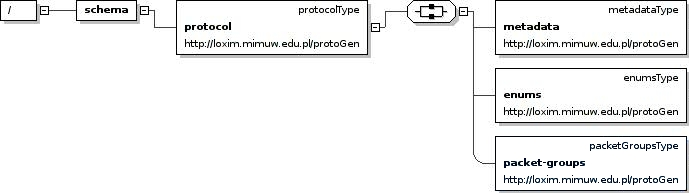
\includegraphics[scale=0.7]{xml/protocol_level.jpg}
		\caption{Konstrukcja znacznika \znacznik{protocol}}
	\end{figure}
	Element \znacznik{protocol} grupuje znaczniki:
	\begin{description}
		\item[\znacznik{metadata}] - opisuj�ce og�lne cechy wygenerowanego protoko�u, a
		tak�e specyficzne cechy zale�ne od docelowego j�zyka programowania.
		\item[\znacznik{enums}] - opisuje typy wyliczeniowe, kt�re mog� zosta� zastosowane
		w protokole. 
		\item[\znacznik{packet-groups}] - opisuje grupy paczek (a zatem te� paczki),
		kt�re, b�d� buduj� protok� bezpo�rednio, b�d� mog� by� elementami sk�adowymi
		paczek. 
    \end{description}

\subsubsection{\znacznik{metadata}}
	\begin{figure}[hbt]
		\centering
			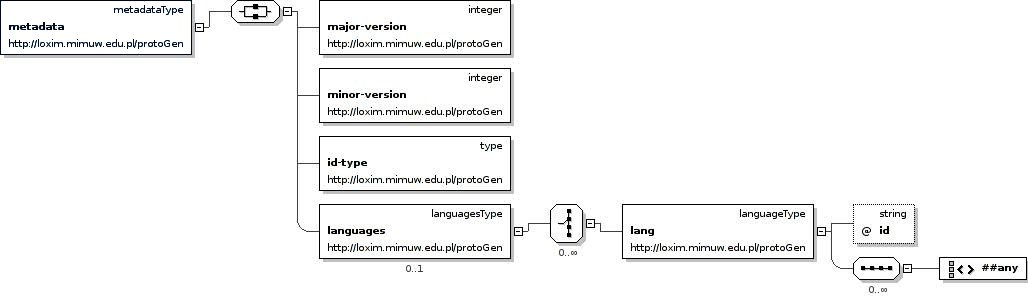
\includegraphics[scale=0.45]{xml/metadata_level.jpg}
		\caption{Konstrukcja znacznika \znacznik{metadata}}
	\end{figure}
	Element \znacznik{metedata} s�u�y opisaniu pewnych og�lnych w�asno�ci protoko�u.
	\begin{description}
		\item[major-version]G��wna wersja protoko�u opisanego w tym deskryptorze.
		Przyjmuje si�, �e protoko�y o tym samym g��wnym numerze wersji s� ze sob�
		kompatybilne (co nie znaczy, �e mo�na za pomoc� nich przekaza� te same
		informacje, ale to �e obie implementacj� b�d� rozmawia�y tak, jakby
		implementowa�y t� sam� - starsz� - wersj� protoko�u). 
		\item[minor-version]Poboczny numer wersji protoko�u.
		\item[languages]Definicja cech protoko�u zale�nych od docelowego j�zyka
		programowania w kt�rym b�dziemy generowali kod. Szczeg�y opisano poni�ej. 
    \end{description}

\subsubsection{\znacznik{lang id="java"}} \label{java-packageName}
	Znacznik ten opisuje dodatkowe atrybuty potrzebne do wygenerowania protoko�u dla j�zyka 
	Java.
		
	\begin{description} 
		\item[packageName]~\\ Nazwa pakietu (jako grupy klas w j�zyku Java)
		zawieraj�cego kod protoko�u. Nale�y oddzieli� wszystkie elementy �cie�ki przy pomocy symbolu '.'. \\
		Wpisana tu nazwa b�dzie tak�e \znacznik{groupId} w utworzonym projekcie Maven2 
		(http://maven.apache.org).
		\item[artifactId]~\\ Nazwa utworzonego modu�u - g��wnie na potrzeby Maven2. 
		\item[version]~\\ Wersja utworzonego modu�u - g��wnie na potrzeby Maven2.  
	\end{description}
	
\subsubsection{\znacznik{lang id="cpp"}}
	J�zyk C++ nie posiada w obecnej wersji ProtoGen dodatkowych atrybut�w. 
	
\subsubsection{\znacznik{enums}} \label{enum}
	\begin{figure}[hbt]
		\centering
			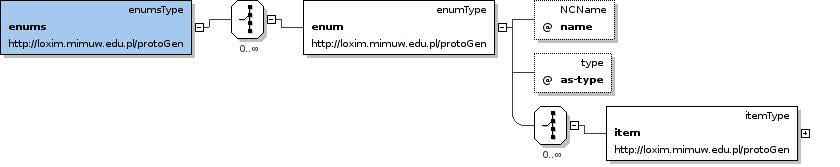
\includegraphics[scale=0.60]{xml/enums.jpg}
		\caption{Konstrukcja znacznika \znacznik{enums}}
	\end{figure}

	Znacznik enums opisuje typy wyliczeniowe, kt�re mog� zosta� wykorzystane w
	protokole. Typy wyliczeniowe mo�na wykorzysta� bezpo�rednio - jako pole 
	zawieraj�ce jedn� warto�� z wielu, a tak�e do stworzenia ,,mapy warto�ci'',
	czyli do przechowania zbioru warto�ci (patrz: \ref{enum-map}). 
	
	\begin{figure}[hbt]
		\centering
			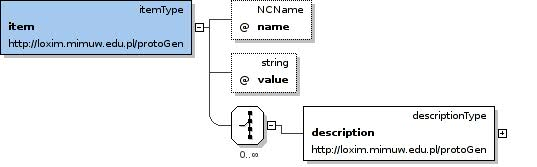
\includegraphics[scale=0.8]{xml/item.jpg}
		\caption{Konstrukcja znacznika \znacznik{item}}
	\end{figure}
	
	Ka�dy element (\znacznik{item}) danego typu wyliczeniowego ma przypisan� warto��
	typu ca�kowitoliczbowego. Je�li chcemy dany typ wyliczeniowy wykorzysta� jako
	,,map�'' to musimy nada� poszczeg�lnym elementom warto�ci o bitach zapalonych
	roz��cznie.
	
	Znacznik \znacznik{enum} opisuje pojedynczy typ wyliczeniowy.
	 
	Jego atrybuty to:
	\begin{description}
		\item[name]    Nazwa typu wyliczeniowego. Przy pomocy tej nazwy b�dzie mo�na
		si� odwo�ywa� do tego typu. Od tej nazwy zale�y te� nazwa wygenerowanej klasy
		przechowuj�cej ten typ. 
		\item[as-type] Nazwa typu numerycznego (patrz: {\ref{typy}}), na kt�ry b�d�
		odwzorcowywane poszczeg�lne enumy. 
    \end{description}

	Ponadto znacznik \znacznik{enum} buduj� elementy \znacznik{item}.  
	
\subsubsection{\znacznik{item}}
	Znacznik item opisuje pojedyncz� warto��, kt�r� mo�e przyj�� typ wyliczeniowy.
	Pojedyncza warto�� posiada nast�puj�ce atrybuty:
	\begin{description}
		\item[name]  Nazwa elementu typu wyliczeniowego.
		\item[value] Warto�� na kt�r� ten element wyliczeniowy b�dzie odwzorowywany.
		Powinna mie�ci� si� w zakresie typu wskazanego w atrybucie ,,as-type'' w znacznika
		\znacznik{enum} definiuj�cym ten typ wyliczeniowy. Warto�� mo�e by� podana
		w systemie dziesi�tnym lub 16-tkowym poprzez poprzedzenie jej symbolami
		,,0x'', np. 0x000f4 - co jest szczeg�lnie przydatne przy konstrukcji typ�w
		u�ywanych do budowania mapy warto�ci (patrz: \ref{enum-map}). 
	\end{description}
	
	Ponadto znacznik \znacznik{item} mo�e posiada� elementy typu \znacznik{description}
	zawieraj�ce dane do budowania dokumentacji (patrz: \ref{description}).

\subsubsection{\znacznik{packet-groups}}
	\begin{figure}[hbt]
		\centering
			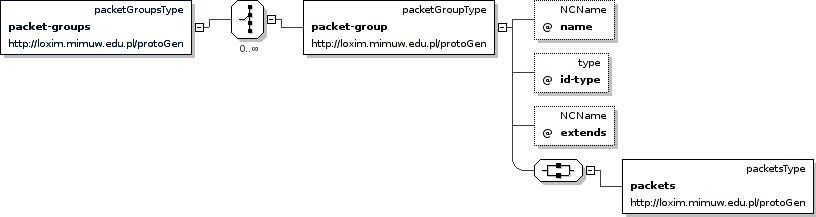
\includegraphics[scale=0.6]{xml/packets_groups_level.jpg}
		\caption{Konstrukcja znacznika \znacznik{packet-groups}}
	\end{figure}

	Znacznik \znacznik{packet-groups} grupuje znaczniki \znacznik{packet-group}, kt�re stanowi� grup�
	paczek. Grupa paczek to taki zbi�r definicji paczek, kt�ra ma r�ne identyfikatory i w podobny
	spos�b jest wykorzystana. W szczeg�lno�ci dla ka�dej grupy paczek zostanie
	wygenerowana fabryka paczek, kt�ra pozwala powo�a� do �ycia paczk� na
	podstawie zadanego jej ,,id''. 
		
	Zawsze powinna istnie� grupa ,,g��wna'' (bez nazwy). Jej elementy b�d�
	stanowi�y podstawowe paczki protoko�u. Pozosta�e (nazwane) grupy s�
	pomocnicze i mog� s�u�y� do budowania p�l innych paczek. 
	
	Grup� charakteryzuj� nast�puj�ce atrybuty: 
	\begin{description}
    	\item[name] - nazwa grupy. Musi istnie� jedna grupa bez nazwy (grupa
    	,,g��wna'')
    	\item[id-type] - nazwa typu ca�kowitoliczbowego(patrz: \ref{typy}),
    	kt�rego typu b�d� identyfikatory paczek. 
    	\item[extend] (atrybut opcjonalny) - nazwa paczki, kt�ra stanowi baz� dla
    	wszystkich paczek tej grupy (o ile nie nadpisano atrybutem extend
    	paczki). Je�li nie zdefiniowano to paczki b�d� dziedziczy�y domy�lnie z
    	g��wnego typu ,,Packet'' nie zawieraj�cego �adnych p�l. 
    \end{description}

	Znacznik \znacznik{packet-group} zawiera podelementy \znacznik{packets}. 

\subsubsection{\znacznik{packets}}
	\begin{figure}[hbt]
		\centering
			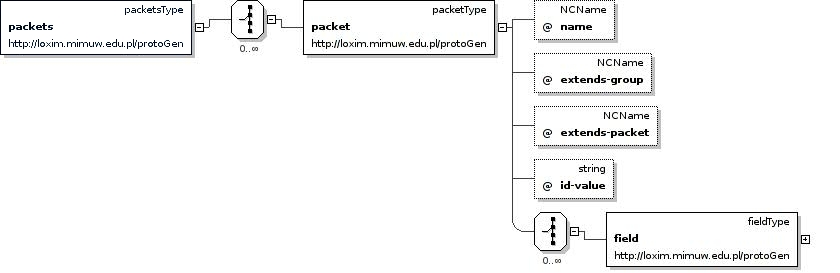
\includegraphics[scale=0.6]{xml/packets_level.jpg}
		\caption{Konstrukcja znacznika \znacznik{packet}}
	\end{figure}

	Element \znacznik{packets} grupuje znaczniki \znacznik{packet}, kt�re opisuj� pojedyncz� paczk�
	danych. Paczka danych sk�ada si� z p�l (patrz: \ref{field}), a ponadto jest
	opisana nast�puj�cymi atrybutami:
	\begin{description}
		\item[name] - Nazwa paczki
		\item[id-value] (atrybut opcjonalny) - Warto�� identyfikuj�ca paczk� (typu
		,,id-type''	z definicji grupy paczek). Je�li paczka nie posiada id-value - to jest
		traktowana jako ,,abstrakcyjna'', co oznacza, �e mo�e by� wykorzystana tylko
		jako paczka bazowa dla innych paczek.
		\item[extends-group] (atrybut opcjonalny) - nazwa grupy paczek, w kt�rej si�
		znajduje si� paczka zdefiniowana w polu ,,extends-packet''.  
		\item[extends-packet] (atrybut opcjonalny) - nazwa paczki z grupy
		''extends-group'', kt�r� deklarowana w�a�nie paczka rozszerza (o dodatkowe pola). 
	\end{description}
	

\subsubsection{\znacznik{field}} \label{field}
	\begin{figure}[hbt]
		\centering
			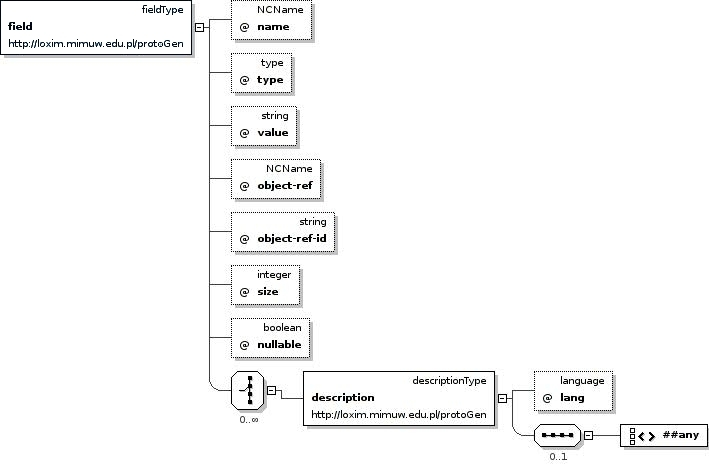
\includegraphics[scale=0.70]{xml/field_level.jpg}
		\caption{Konstrukcja znacznika \znacznik{fields}}
	\end{figure}

	Znacznik \znacznik{field} opisuje pojedyncze pole paczki. Podelementem znacznika \znacznik{field}
	mo�e by� znacznik \znacznik{description} (patrz: \ref{description}). Atrybutami znacznika
	field niezale�nie od typu tego pola s�:
	\begin{description}
		\item[name] - Nazwa pola
		\item[type] - Typ pola (patrz: \ref{typy})
	\end{description}

	Pozosta�e atrybuty zale�� od typu pola:
	\begin{itemize}
	\item Dla typ�w prostych dost�pny jest dodatkowo atrybut ,,value'' mog�cy
	zawiera� domy�ln� zawarto�� pola. 

	\item Dla typ�w: string, sstring, varuint dost�pny jest atrybut ''nullable''
	(przyjmuj�cy warto�ci true lub false), �wiadcz�cy o tym, czy dopuszczalna jest
	zawarto�� NULL dla tego pola. 
	
	\item Dla typ�w: string i sstring dost�pny jest atrybut size zawieraj�cy
	maksymaln� dopuszczaln� d�ugo�� napisu. 
	\end{itemize}
	
	Ponadto nast�puj� typy z�o�one wymagaj� szczeg�lnego om�wienia:
	\begin{description}
		\item[enum] - Pole zawiera jedn� z warto�ci z listy wyboru. Atrybut
		,,object-ref'' wskazuj� na nazw� odpowiedniego ,,enuma'' (patrz: \ref{enum}).
		Pole b�dzie serializowane jako typ ca�kowitoliczbowy wskazany w definicji
		,,enuma'' o warto�ci odpowiadaj�cej ,,id'' wybranego elementu z tej listy
		wyboru.
		\item[enum-map] \label{enum-map} - Pole zawiera bitow� map� warto�ci w listy
		wyboru. Atrybut ,,object-ref'' wskazuj� na nazw� odpowiedniego ,,enuma'' (patrz: \ref{enum}).
		Pole b�dzie serializowane jako typ ca�kowitoliczbowy wskazany w definicji
		,,enuma'' o warto�ci odpowiadaj�cej sumie ,,id'' wybranych elementu z tej
		listy wyboru.
		\item[package] - Pole zawiera cia�o (bez nag��wka) ca�ej innej paczki.
		Atrybut ,,object-ref'' wskazuj� na nazw� grupy paczek, a ,,object-ref-id'' na
 		nazw� konkretnej paczki nale��cej do tej grupy.
		\item[package-map] - Pole zawiera cia�o ca�ej innej paczki nale��cej
		do wskazanej grupy paczek, ale konkretny rodzaj paczki jest wyznaczony przez
		warto�� innego - uprzednio wymienionego pola. Zatem ,,object-ref'' wskazuj�
		na nazw� grupy paczek, a ,,object-ref-id'' na nazw� wcze�niej
		zdefiniowanego pola w bie��cej paczce - kt�re b�dzie zawiera�o
		identyfikator paczki, kt�ry ma zosta� w bie��cym polu wczytany/zapisany.
		O polu ,,package-map'' nale�y my�le� jak o polu ,,package'' z dynamicznie
		wyznaczanym konkretnym rodzajem paczki. 
    \end{description}
	
		
	
\subsubsection{\znacznik{description}}\label{description}
	Znacznik \znacznik{description} mo�e wyst�powa� w wielu miejscach specyfikacji
	protoko�u. S�u�y on do wygenerowania dokumentacji dotycz�cej wskazanego
	elementu protoko�u. Znacznik ten zawiera atrybut ,,lang'', kt�rego warto�ci�
	powinien by� kod j�zyka (kraju) - dwuliterowy, opisuj�cy j�zyk w kt�rym zosta�
	przeprowadzony opis. Zawarto�ci� znacznika mo�e by� dowolny tekstem tak�e
	wzbogacony o znaczniki j�zyka HTML. 

\subsubsection{Schemat (XML Schema) deskryptora protoko�u} \label{xml-schema}
\lstset{language=xml,tabsize=2,breaklines=true,showspaces=false,showstringspaces=false,showtabs=false}
\lstinputlisting{protogen.xsd}

\subsection{Proste typy danych}\label{typy}

	\subsubsection{Postanowienia og�lne}
		\begin{itemize}
          \item Je�li w spos�b szczeg�lny nie zaznaczono inaczej (a raczej
          nigdzie nie zaznaczono) wszystkie warto�ci zapisywane s� w formacie
          Big-endian.  W szczeg�lno�ci obejmuje to typy ca�kowitoliczbowe,
          rzeczywiste, oraz napisy w kodowaniu UTF-8 tak�e stosuj� kolejno��
          Big-endian. 
        \end{itemize}               

 	 \subsubsection{Ca�kowitoliczbowe: uint8,  sint8, uint16, sint16, int32,
 	 uint32, uint64, sint64} \label{integers}
		
	Pierwsza litera determinuje, czy mamy do czynienia z typem ze znakiem (u -
	unsigned), czy z typem bez znaku (s - signed).  Liczba na ko�cu wyra�a d�ugo��
	typu wyra�on� w bitach. 
	
	Typy s� kodowane oczywi�cie w kolejno�ci Big-endian. 
		
	\subsubsection{varuint - Ca�kowitoliczbowy z kompresj� (1,3,5 lub 9 bajt�w)}
		B�dzie to typ u�ywany g��wnie do oznaczania d�ugo�ci string�w i paczek. 
		
		Rozwi�zanie techniczne zosta�o zaczerpni�te z protoko�u serwera MySQL
		\cite{MySQL}.
		
		Idea jest taka, �e kr�tkie stringi ($<250$znak�w ) b�d� si�
		pojawia�y najcz�ciej i chcemy mie� najmniejszy narzut na zapisanie d�ugo�ci
		(jedno bajtowy). 
		
		Zatem semantyka pierwszego bajtu jest nast�puj�ca (w zale�no�ci od jego
		warto�ci)
		\begin{description}
			\item[0-249] Warto�� ta jest jednocze�nie warto�ci� wynikow�
			\item[250] Warto�� jest null'em (zostawiamy dla umo�liwienia stosowanie
			tego rozwi�zania z systemami relacyjnymi) 
			\item[251] Warto�� ta poprzedza 2-bajtowe (uint16) pole w warto�ci� w�a�ciw�
			\item[252] Warto�� ta poprzedza 4-bajtowe (uint32) pole z warto�ci� w�a�ciw�
			\item[253] Warto�� ta poprzedza 8-bajtowe (uint64) pole z warto�ci�
			w�a�ciw�. Nie nale�y jednak korzysta� z warto�ci wi�kszych ni� $2^{63}-1$
			(MAX\_SINT64), ze wzgl�du na to, �e w Javie nie s� obs�ugiwane 8 bajtowe
			typy bez znaku. 
        \end{description}
	
	\subsubsection{string - �a�cuchy tekstu}
	
	S�u�y do przesy�ania tekst�w. Teksty te musz� by� kodowane za pomoc� UTF-8. 
	
	Format warto�ci typu string jest nast�puj�cy:
	Najpierw idzie pole typu varuint - opisuj�ce d�ugo�� w bajtach nast�puj�cego
	potem ci�gu w UTF-8 (Big-endian). 
	
	\subsubsection{sstring - Kr�tki �a�cuch tekstu}
	Jest to tak naprawd� wariant typu string, 
	ale ograniczony do �a�cuch�w nie d�u�szych ni� 249 bajt�w.
	Czyli wtedy pole oznaczaj�ce d�ugo�� ma jeden bajt. 
	Jego wewn�trzna reprezentacja zupe�nie si� nie r�ni od typu
	string - zosta� on wyr�niony formalnie - ze wzgl�du na uproszczenie notacji 
	u�ywanej przy opisach format�w poszczeg�lnych paczek, a tak�e ze wzgl�d�w
	bezpiecze�stwa - gdy� pozwala zmniejszy� ryzyko typu DOS poprzez zaw�enie 
	wielko�ci danych, kt�re mog� by� zinterpretowane przez serwer. 
	
	\subsubsection{bytes - Dane binarne}\label{bytes}
	S�u�y do przesy�ania danych binarnych (tablic bajt�w).  
	
	Format warto�ci typu bytes jest nast�puj�cy:
	Najpierw jest wysy�ane pole typu varuint - opisuj�ce d�ugo�� w bajtach
	nast�puj�cego potem ci�gu bajt�w.
	
\newpage
\section{Dokumentacja wygenerowanego kodu}

\subsection{Wygenerowany kod dla j�zyka Java}
Generator protoko��w generuje kod w j�zyku Java w wersji nie starszej ni� Java
1.5, poniewa� korzysta z typ�w wyliczeniowych (enums) i szablon�w (generics). 

Zak�adaj�c, �e w metadanych opisu protoko�u dla j�zyka java zadeklarowano
packageName jako 'taki.sobie.protokol' (patrz: \ref{java-packageName}) to
zostanie wygenerowany nast�puj�cy projekt:

\subsubsection{pom.xml}
Pom.xml (Project Object Model) jest to plik opisuj�cy jak kompilowa� ten modu�
za pomoc� narz�dzia ,,Maven2''. Wskazuje on w szczeg�lno�ci biblioteki od
kt�rych projekt zale�y. 

\hyphenation{lo-xim}
\hyphenation{ja-va}
\hyphenation{pro-to-lib}

Modu� protoko�u wygenerowany przez ProtoGen zale�y od
biblioteki: \\pl.edu.mimuw.loxim.protogen.lang.java.protolib:java\_protolib, kt�ra
zawiera definicj� odpowiednich strumieni i klas bazowych (patrz:
\ref{java-protolib}).

Aby zbudowa� modu� wystarczy (zak�adaj�c, �e u�ytkownik posiada zainstalowanego Maven'a 2
\footnote{http://maven.apache.org/download.html}) wykona� polecenie ,,mvn package'' w
katalogu zawieraj�cym plik pom.xml. Wyniki procesu budowania zostan�
umieszczone w katalogu target. 

\subsubsection{Typy wyliczeniowe - enumy}
	Ka�dy ,,enum'' (typ wyliczeniowy) zostanie zapisany do katalogu
	./src/main/java/taki/sobie/protokol/enums jako ,,Enum'' j�zyka Java
	(wersja 1.5+).
	
	Typ ,,enum-map'' jest odwzorcowywany na odpowiedni ,,java.util.EnumSet$<$typ
	bazowy$>$'' (patrz: \ref{enum-map}).

\subsubsection{Grupy paczek} \label{java-PackagesFactory}

Paczki grupy g��wnej zostan� zapisane w folderze
./src/main/java/taki/sobie/protokol/packages, a paczki z pozosta�ych grup w 
folderze ./src/main/java/taki/sobie/protokol/packages\_$[$nazwa\_grupy$]$.

W ka�dym takim folderze powstanie tak�e klasa b�d�ca fabryk� paczek, 
kt�ra udost�pnia metod�:\\ 

public Package createPackage(long package\_id) throws
ProtocolException\\ 

Metoda ta tworzy paczk� w zale�no�ci od danego identyfikatora
paczki.

\subsubsection{Paczki} \label{java-paczki}

Dla ka�dej paczki zadeklarowanej w opisie protoko�u jest tworzona
odpowiednia klasa paczki. Wszystkie paczki rozszerzaj� nast�puj�c� klas�: 

\lstset{language=java,tabsize=2,breaklines=true,showspaces=false}
\lstinputlisting{src/Package.java}

Ponadto ka�da paczka zawiera nast�puj�ce elementy:
\begin{itemize}
  \item Publiczn� sta�� ID zawieraj�c� identyfikator paczki
  \item Bezparametrowy konstruktor paczki
  \item Konstruktor paczki, kt�ry przyjmuje wszystkie pola paczki jako swoje
  parametry
  \item Gettery i settery dla wszystkich p�l paczki 
\end{itemize}

\subsubsection{Testy}

Generator wygeneruje tak�e testy:
\begin{description}
  \item[./src/test/java/taki/sobie/protokol/tests/TestRunnerRec.java] - \\ 
  Klasa j�zyka java daj�ca si� uruchomi� (zawiera metod� main), kt�ra uruchamia
  proces, kt�ry otwiera gniazdo TCPIP na wskazanym porcie i sprawdza, czy
  otrzymane paczki s� zgodne z oczekiwanymi. Jedynym parametrem jaki mo�na
  przekaza� uruchamiaj�c t� klas� jest numer portu na kt�rym chcemy otworzy�
  gniazdo serwera. 
  
  Program ten mo�na wykorzystywa� do test�w komunikacji z implementacjami
  protoko�u dla innych j�zyk�w programowania.  
  
  \item[./src/test/java/taki/sobie/protokol/tests/TestRunnerSender.java] - \\
  Klasa j�zyka java daj�ca si� uruchomi� (zawiera metod� main), kt�ra uruchamia
  proces, kt�ry wysy�a na wskazany port na wskazanym serwerze paczki testowe.
  Uruchamiaj�c musimy przekaza� dwa parametry: nazw� hosta docelowego (lub
  adres IP), a tak�e port do kt�rego chcemy si� pod��czy�. 
  
  Program ten mo�na wykorzystywa� do test�w komunikacji z implementacjami
  protoko�u dla innych j�zyk�w programowania. 
   
  \item[./src/test/java/taki/sobie/protokol/tests/TestPackagesFactory.java] -\\
  Zawiera konstruktor wygenerowanych paczek testowych. Stanowi baz� dla
  innych test�w. 
  \item[./src/test/java/taki/sobie/protokol/tests/TestPackages.java] -\\
  Jest JUnitowym testem, kt�ry zapisuje wszystkie paczki testowe do
  strumienia, a nast�pnie je wszystkie wczytuje i sprawdza, czy paczki s�
  r�wne. Ten test jest u�ywany w fazie test�w w procesie budowania modu�u
  przez Maven 2. 
\end{description}

\subsubsection{java\_protolib}\label{java-protolib}
Biblioteka java\_protolib.jar jest plikiem, kt�ry zawiera niezale�n� od
konkretnego protoko�u definicj� podstawowych klas i interfejs�w.  

Poni�ej listujemy kluczowe klasy znajduj�ce si� w tej bibliotece: 

\begin{description}
\item[pl.edu.mimuw.loxim.protogen.lang.java.template.layers.ProtocolLayer0]~\\
Podstawowa klasa u�ywana w aplikacji do obs�ugi protoko�u. Zawiera metody
wysy�aj�ce przekazan� paczk�, a tak�e czekaj�c� i odczytuj�c� paczk�. Klasa
ponadto automatycznie odpowiada na paczk� ,,Ping'' paczk� ,,Pong''. 

\item[pl.edu.mimuw.loxim.protogen.lang.java.template.exception.ProtocolException]~\\
Wyj�tek rzucany gdy co� w protokole p�jdzie nie tak jak powinno. 

\item[pl.edu.mimuw.loxim.protogen.lang.java.template.pstreams.PackageOutputStream]~\\
Strumie� zak�adany na OutputStream'ie, kt�ry udost�pnia metod�
writePackage(Package p).

\item[pl.edu.mimuw.loxim.protogen.lang.java.template.pstreams.PackageInputStream]~\\
Strumie� zak�adany na InputStreamie, kt�ry udost�pnia metod� readPackage().

\item[pl.edu.mimuw.loxim.protogen.lang.java.template.streams.PackageOutputStreamWriter]~\\
Strumie� zak�adany na OutputStream'ie, kt�ry udost�pnia metody pozwalaj�ce
zapisa� proste typy danych (patrz \ref{typy}). 

\item[pl.edu.mimuw.loxim.protogen.lang.java.template.streams.PackageInputStreamReader]~\\
Strumie� zak�adany na InputStream'ie, kt�ry udost�pnia metody pozwalaj�ce
odczyta� proste typy danych (patrz \ref{typy}). 

\item[pl.edu.mimuw.loxim.protogen.lang.java.template.auth.AuthPassMySQL]~\\
Klasa pomocnicza oferuj�ca wsparcie dla przeprowadzania autoryzacji tak� metod�
jak robi to serwer bazy danych MySQL (,,Password Algorithm'' \cite{MYSQL})

\item[pl.edu.mimuw.loxim.protogen.lang.java.template.pstreams.PackagesFactory]~\\
Interfejs, kt�ry implementuj� wszystkie fabryki pakiet�w (patrz:
\ref{java-PackagesFactory})

\item[pl.edu.mimuw.loxim.protogen.lang.java.template.ptools.Package]~\\
Klasa bazowa dla wszystkich paczek.
\end{description}


\subsection{Wygenerowany kod dla j�zyka C++}
Kod dla j�zyka C++ jest samodzielny (jedyn� zale�no�ci� jest OpenSSL potrzeby
do dzia�aj�cej autoryzacji metod� zastosowan� w serwerze MySQL). Buduje si� go
za pomoc� polecenia make wydanego w katalogu ,,protocol''. 

\subsubsection{./make.defs}
Zawiera definicj� narz�dzi i bibliotek u�ywanych przez make. 

\subsubsection{Autentykacja - ./protocol/auth}
W tym folderze zawarte s� klasy pomocnicze potrzebne do 
przeprowadzenia autentykacji. Obecnie zaimplementowana jest tylko klasa
AuthPassMySQL wspieraj�ca autentykacj� metod� zastosowan� w serwerze MySQL i
wykorzystuj�ca sumy kontrolne SHA1. 

\subsubsection{Strumienie paczek - ./protocol/pstreams}

PackageOutputStream - Strumie� zak�adany na OutputStream;ie, kt�ry udost�pnia
metod� writePackage(Package* p).

PackageInputStream - Strumie� zak�adany na InputStream'ie, kt�ry udost�pnia
metod� readPackage() wczytuj�c� dany pakiet ze strumienia. 

\subsubsection{Typy wyliczeniowe - ./protocol/enums}
Ka�dy typ wyliczeniowy definiuje odpowiedni ,,enum'' j�zyka C++. 
Tworzony jest tak�e typ mapy (zawieraj�cy pole bitowe dla ka�dej warto�ci typu
wyliczeniowego). 

Ponadto tworzona jest tak�e fabryka umo�liwiaj�ca stworzenie instancji enuma lub
mapy enum�w na podstawie przekazanej warto�ci ca�kowitej, a tak�e zapisanie
enuma lub mapy enum�w jako liczb�. 

\subsubsection{Grupy pakiet�w}

Paczki grupy g��wnej zostan� zapisane w katalogu: ./protocol/packages, 
a grup nazwanych w ./protocol/packages\_$[$nazwa\_grupy$]$.

Dla ka�dej grupy zostanie wygenerowana klasa, b�d�ca fabryk� paczek w
zale�no�ci od przekazanego identyfikatora paczki. 

\subsubsection{Paczki}

Dla ka�dej paczki zostaje zaimplementowana klasa analogiczna do tej opisanej 
dla j�zyka Java (patrz: \ref{java-paczki}). 


\subsubsection{Testy - ./protocol/tests}
\begin{description}
	\item[./protocol/tests/TestRunnerRec]
	Uruchamia
  proces, kt�ry otwiera gniazdo TCPIP na wskazanym porcie i sprawdza, czy
  otrzymane pakiety s� zgodne z oczekiwanymi. Jedynym parametrem jaki mo�na
  przekaza� uruchamiaj�c t� klas� jest numer portu na kt�rym chcemy otworzy�
  gniazdo serwera. 
  
  Program ten mo�na wykorzystywa� do test�w komunikacji z implementacjami
  protoko�u w innych j�zykach programowania.  

	\item[./protocol/tests/TestRunnerSender]
	 Uruchamia
  proces, kt�ry wysy�a na wskazany port na wskazanym serwerze pakiety testowe.
  Uruchamiaj�c musimy przekaza� dwa parametry: nazw� hosta docelowego (lub
  adres IP), a tak�e port do kt�rego chcemy si� pod��czy�. 
  
  Program ten mo�na wykorzystywa� do test�w komunikacji z implementacjami
  protoko�u w innych j�zykach programowania. 

	\item[./protocol/tests/TestPackagesFactory]
  Jest to fabryka wygenerowanych pakiet�w testowych. Stanowi baz� dla
  innych test�w. 
\end{description}

\subsubsection{Gniazda - ./protocol/sockets}
Katalog zawiera prost�, obiektow� implementacj� gniazd. Jest ona wzorowana na
tej dost�pnej w j�zyku Java i umo�liwia �atwe u�ywanie gniazd sieciowych (zar�wno
serwerowych jak i klienckich) i otwieranie strumieni na nich. 

\begin{itemize}
\item ./protocol/sockets/TCPIPServerSocket
\item ./protocol/sockets/TCPIPServerSingleSocket
\item ./protocol/sockets/AbstractSocket
\item ./protocol/sockets/TCPIPClientSocket
\end{itemize}

\subsubsection{Strumienie ./protocol/streams}
Katalog zawiera elementarne, obiektowe implementacje strumieni - wzorowane na
j�zyku Java. 

\begin{description}
  \item[./protocol/streams/AbstractOutputStream,AbstractInputStream] -
  abstrakcyjne klasy bazowe dla strumieni
  \item[./protocol/streams/DescriptorInputStream,DescriptorOutputStream] -
  prosta implementacja strumieni oparta o zapis i odczyt ze wskazanego
  deskryptora systemu operacyjnego (pliku, urz�dzenia, gniazda sieciowego,
  ��cza). 
  \item[./protocol/streams/PriorityOutputStream]
  Klasa okalaj�ca (wrapper) strumienia wyj�ciowego, kt�ry udost�pnia dodatkow�
  metod� writePriority(char*), kt�ra przy wielu odwo�aniach do tego obiektu (z
  wielu w�tk�w) zostanie wykonana przed wykonaniami zapisu w zwyk�ych metodach
  write(char*) (odpowiednia synchronizacja na semaforach). 
\end{description}

\subsubsection{Warstwy protoko�u - ./protocol/layers/ProtocolLayer0}
Podstawowa klasa u�ywana w aplikacji do obs�ugi protoko�u. Zawiera metody
wysy�aj�ce przekazan� paczk�, a tak�e metod� czekaj�c� na i odczytuj�c� paczk�.
Klasa ponadto automatycznie odpowiada na paczki ,,Ping'' paczkami ,,Pong''. 

\subsubsection{Klasy pomocnicze}

\begin{description}
\item[./protocol/ptools/Endianness] -\\ 
Klasa zawiera metody u�atwiaj�ce konwersj� Little/Big Endian dla typ�w prostych
\item[./protocol/ptools/StringBufferStack] -\\
Klasa umo�liwia szybk� konstrukcje napis�w (bufor�w znak�w) poprzez sklejanie
napis�w (tablic znak�w). 
\item[./protocol/ptools/Package] -\\
Klasa bazowa dla wszystkich paczek
\item[./protocol/ptools/CharArray] -\\
Tablica znak�w z okre�lonym rozmiarem 
\item[./protocol/ptools/PackageBufferWriter] -\\
Klasa zawieraj�ca metody zapisuj�ce do danego strumienia typy proste. 
\item[./protocol/ptools/PackageBufferReader] -\\
Klasa zawieraj�ca metody odczytuj�ce z danego strumienia typy proste.
\end{description}

\subsubsection{Przyk�adowy kod u�ywaj�cy protok� po stronie serwera}

\lstset{language=C++,tabsize=2,breaklines=true,showspaces=false}
\lstinputlisting{src/UsageExampleServer.cpp}


\subsubsection{Przyk�adowy kod u�ywaj�cy protok� po stronie klienta}

\lstset{language=C++,tabsize=2,breaklines=true,showspaces=false}
\lstinputlisting{src/UsageExampleClient.cpp}

\newpage
\section{Dokumentacja programistyczna}
	\subsection{Architektura rozwi�zania}
		\subsubsection{Java}
ProtoGen zosta� napisany w j�zyku Java co umo�liwia u�ywanie go na wi�kszo�ci
platform sprz�towych i z wykorzystaniem wielu system�w operacyjnych.
 
		\subsubsection{Plexus - zorientowana na komponenty}
ProtoGen zosta� napisany w architekturze zorientowanej na komponenty. Do
zarz�dzania komponentami u�ywamy biblioteki Plexus (http://plexus.codehaus.org).
Z punktu widzenia u�ytkownika i programisty, zastosowanie tej architektury
umo�liwia stosunkowo �atwe dodanie obs�ugi nowego j�zyka generowanego kodu.
Wymaga ono jedynie stworzenia implementacji interfejsu:
,,pl.edu.mimuw.loxim.protogen.api.PartialLanguageGenerator'', a nast�pnie zadeklarowanie jej w
 lokalnym deskryptorze components.xml jar'a zawieraj�cego t� implementacj� jako: 

\lstset{language=xml,tabsize=2,breaklines=true,showspaces=false,showstringspaces=false,showtabs=false}
\lstinputlisting{src/components.xml}


W momencie, gdy taki jar znajdzie si� w classpath'ie uruchamianego ProtoGen'a,
to j�zyk ,,NowyJ�zyk'' b�dzie dost�pny jako jeden z docelowych j�zyk
dla generowanego kodu.

Reasumuj�c, g��wn� korzy�ci� zastosowania architektury zorientowanej na
komponenty, jest umo�liwienie zewn�trznym dostawcom dodawanie implementacji
nowych j�zyk�w bez �adnej ingerencji w dost�pny dotychczas kod. 
		
	\subsection{Proces budowania aplikacji}
	
	\begin{enumerate}
      \item Zainstalowa� Maven2 (http://maven.apache.org/download.html)
      \item Wej�� do katalogu g��wnego ProtoGen'a i wyda� polecenie ,,mvn
      clean package assembly:assembly''
      \item W podkatalogu ,,target/protogen-x.xx.xx-bin.dir'' b�dzie si�
      znajdowa�a wersja dystrybucyjna projektu. 
    \end{enumerate}
	
\subsection{Dalszy rozw�j} \label{roadmap}
	
	\subsubsection{Z�o�ona logika}
	Obecnie ProtoGen nie wspiera z�o�onej logiki w konstrukcji pakiet�w. Niemo�liwe jest warunkowanie istnienia pola w zale�no�ci od warto�ci innego pola,
	a tak�e tworzenia tablicy p�l. Obecnie ProtoGen przewiduje mo�liwo��
	nadpisania wygenerowanego kodu. W ten spos�b mo�na - nadpisuj�c kod obs�ugi
	odpowiedniej paczki - uzyska� obs�ug� dowolnie z�o�onej logiki.
		 	
	�eby zminimalizowa� konieczno�� wykorzystania takiego obej�cia, a tym
	samym uzyska� ,,pe�no��'' rozwi�zania przewidujemy w przysz�ych wersjach
	mo�liwo�� wprowadzenia nast�puj�cych atrybut�w do pola field (patrz:
	\ref{field}):
	\begin{description}
		\item[if-field] --- Zawiera nazw� pola z bie��cej paczki (wcze�niej
		zadeklarowanego), kt�rego warto�� b�dziemy por�wnywali do ,,if-value''. 
		\item[if-value] --- Je�eli zawarto�� pola o nazwie zadanej atrybutem ,,if-field''
		jest r�wna warto�ci ,,if-value'' to opisywane pole wyst�puje w tej paczce. W
		przeciwnym przypadku nie wyst�puje.
		\item[repeat] --- Zawiera nazw� pola ca�kowitoliczbowego, kt�re zawiera
		informacj� ile razy bie��ce pole jest powt�rzone.  
    \end{description}
	
	\subsubsection{Wi�cej j�zyk�w programowania}

	System jest przystosowany do rozszerzania o generatory do innych j�zyk�w
	programowania bez modyfikacji kodu �r�d�owego projektu bazowego. Dodanie
	obs�ugi nowego j�zyka programowania wymaga napisania komponentu systemu Plexus
	implementuj�cego interfejs
	,,pl.edu.mimuw.loxim.protogen.api.PartialLanguageGenerator''. 
	
	Oczywistym jest, �e dodanie generator�w do j�zyk�w programowania takich jak,
	C\#, Python, Ruby, PHP, Ocaml istotnie zwi�kszy u�yteczno�� tego projektu. 
	\subsubsection{Generowanie dokumentacji}
	Podobnie jak z dodatkowymi j�zykami programowania, wydaje si� istotn� z punktu
	widzenia u�ytkownika mo�liwo�� uzyskania aktualnej dokumentacji protoko�u.
	Cech� po��dan� jest by ProtoGen by� wstanie wygenerowa� dokumentacj� -
	najlepiej do wielu najpopularniejszych format�w (HTML, \LaTeX, PDF, ODF).
	
	By unikn�� r�cznej obs�ugi tych wszystkich format�w - wydaje si� uzasadnionym
	u�ycie narz�dzia typu Doxia (http://maven.apache.org/doxia), kt�re umo�liwia
	konwersje pomi�dzy wieloma formatami ,,bogatego'' tekstu.
	
	\subsubsection{Wsparcie dla wielu wersji pobocznych}
	
	Zar�wno definicj� paczki, jak i pola mo�na rozszerzy� o atrybut
	,,since-minor-version'', kt�ry b�dzie specyfikowa� od kt�rej wersji pobocznej
	protoko�u dane pole wyst�puje.
	
	Dodatkowo wymagamy, by kolejno��
	warto�ci ,,since-minor-version'' zgadza�a si� z kolejno�ci� p�l w paczce i by
	ka�de pole posiadaj�ce ten atrybut posiada�o tak�e zadeklarowan� warto��
	domy�ln� (pole ,,value''). Warunki te s� wystarczaj�ce, by zachowa� zgodno��
	protoko�u pomi�dzy r�nymi wersjami pobocznymi.  



	\begin{thebibliography}{}
		\bibitem[1]{MySQL}MySQL Protocol - version 10. Ian Redfern,
		[03.12.2006], (http://www.redferni.uklinux.net/mysql/MySQL-Protocol.html) 
	\end{thebibliography}

\end{document}
